\documentclass[12pt]{article}
\input{preamble}

\pagestyle{fancy}
\fancyhf{}

\rhead{Nørre Gymnasium\\
1.x
}


%Husk at rette modul og dato!
\lhead{Matematik A\\
	Polynomier
}
\chead{10. april 2026
}

\cfoot{Side \thepage \hspace{1pt} af \pageref{LastPage}}

\begin{document}

%Udfyld afsnit herunder og lav til egen Latex-fil

%Kopier følgende til overskrift:

%\begin{center}
%\Huge
%Aflevering 1
%\end{center}
%\section*{Opgave 1}
%\stepcounter{section}
%Overskrift

%\begin{center}
%\Huge
%Aflevering 1
%\end{center}



\begin{center}
	\Large Uden hjælpemidler
\end{center}

\subsection*{Opgave 1}
\begin{center}
		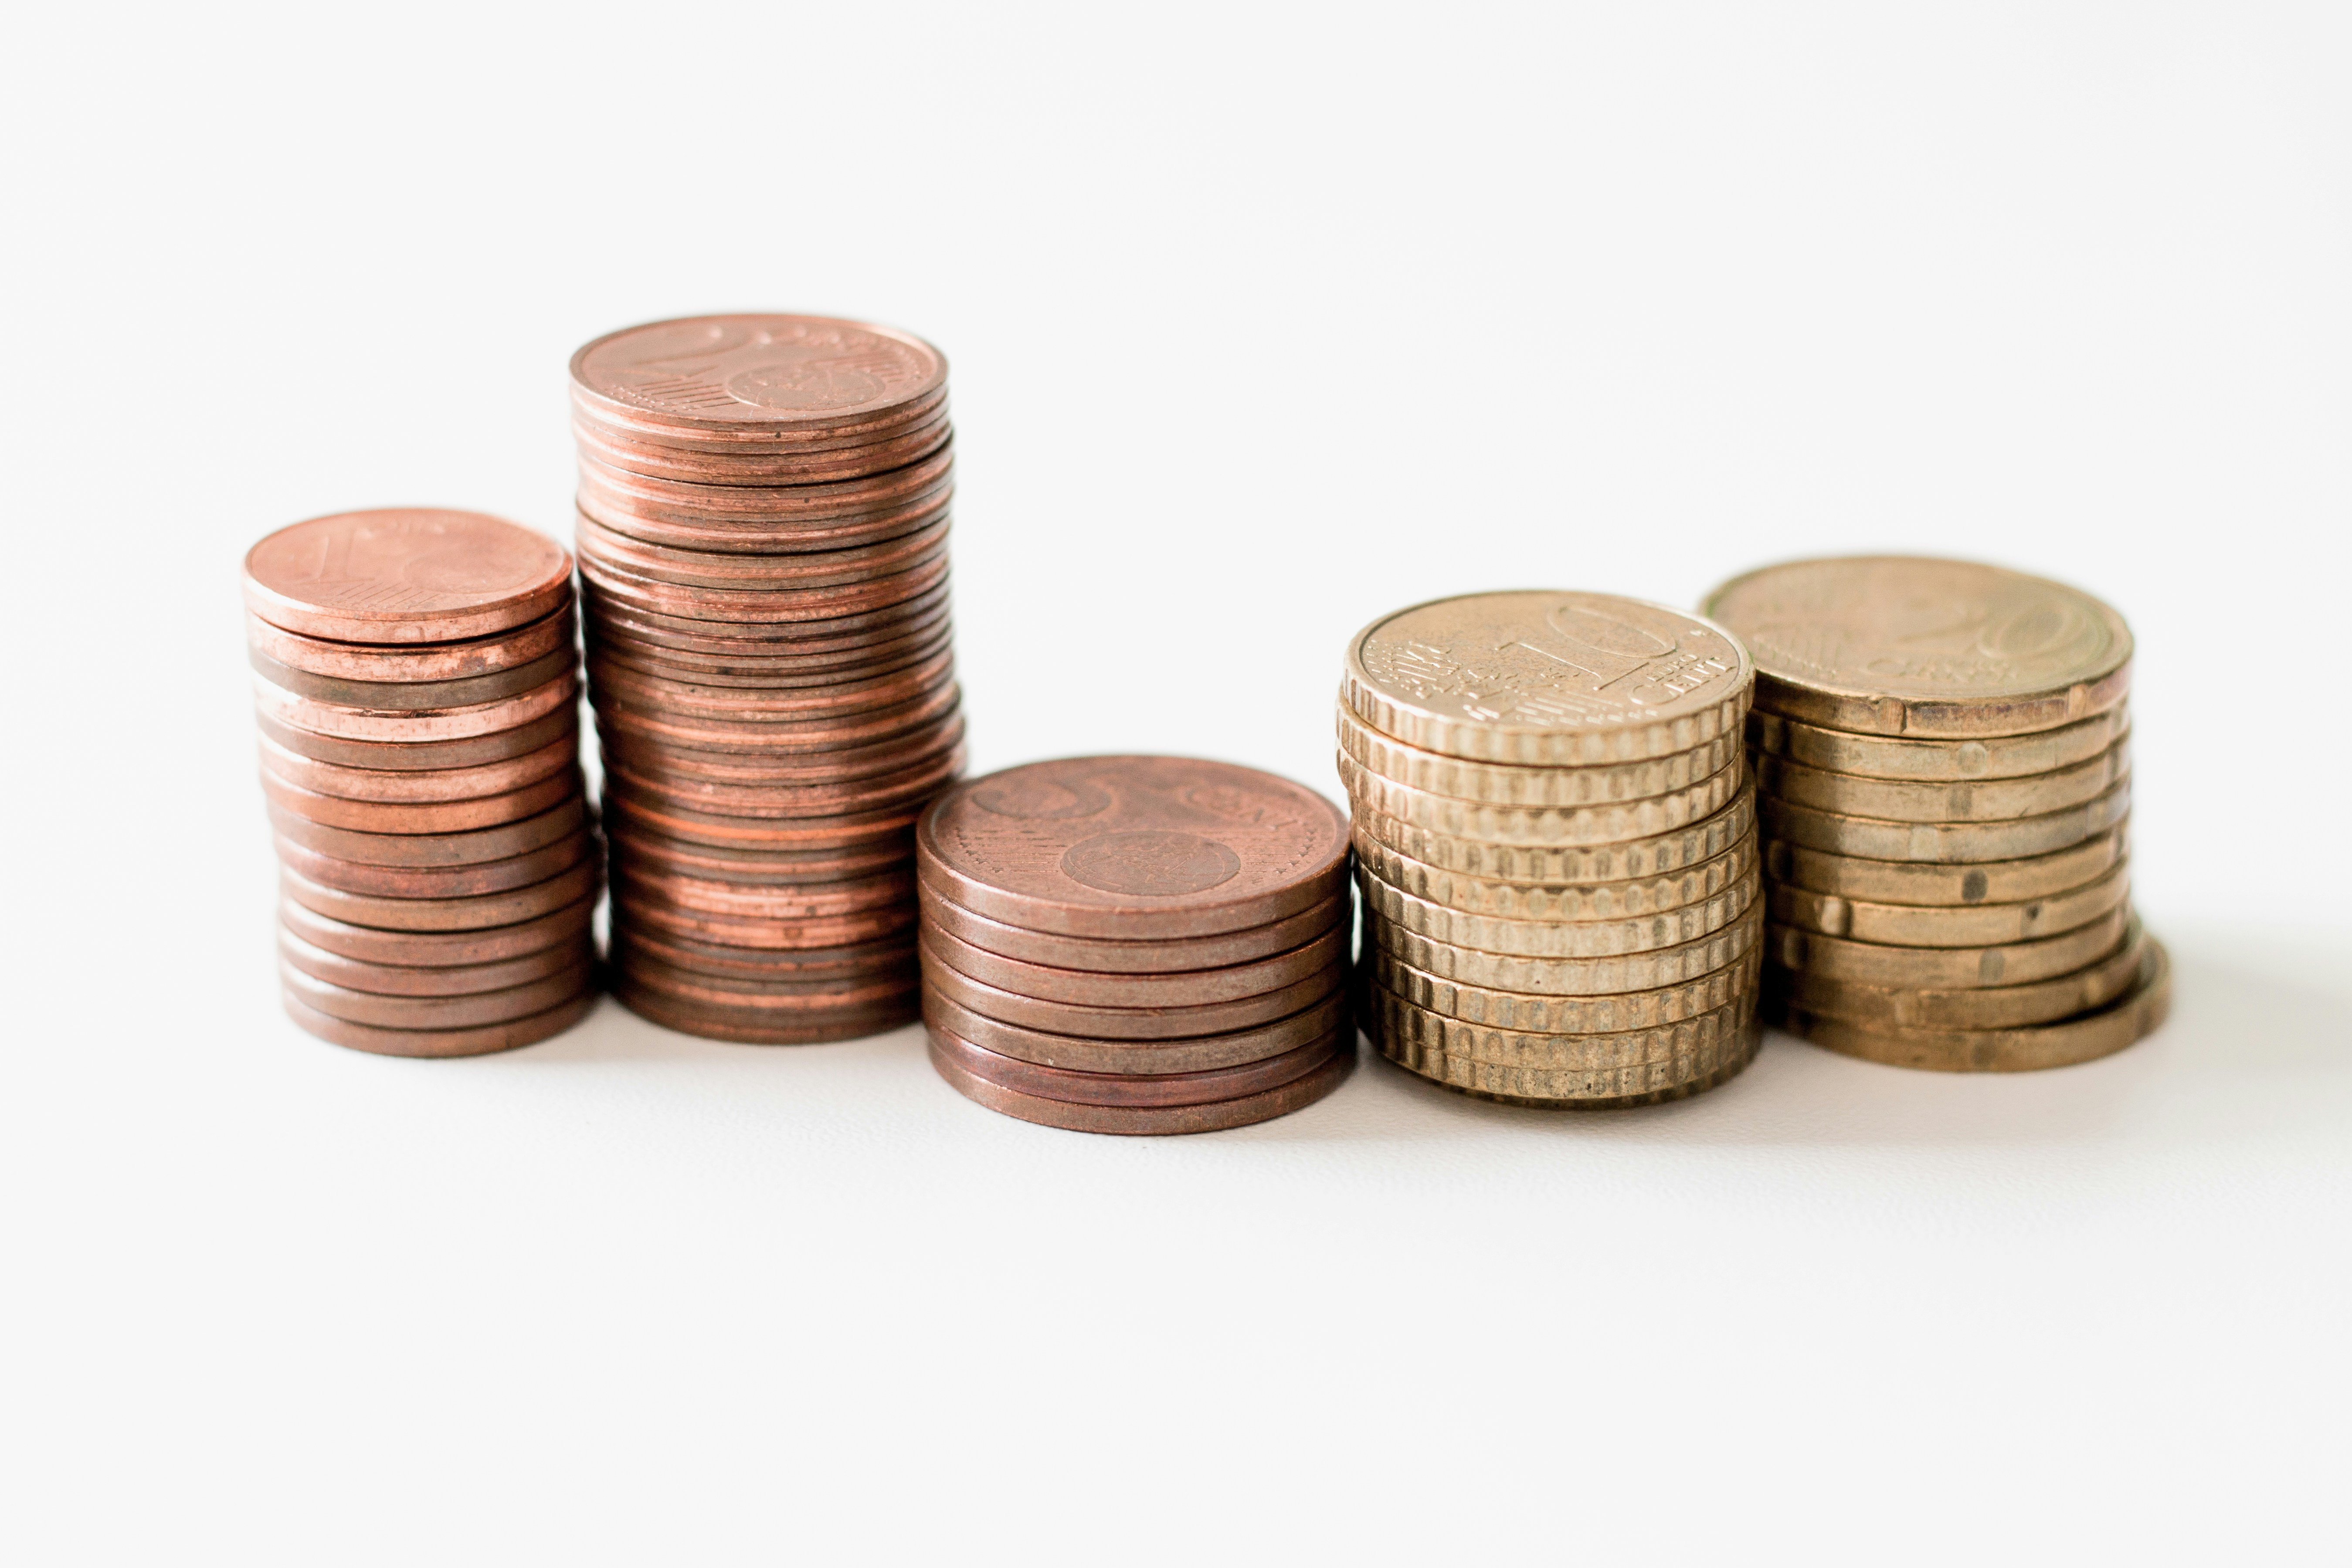
\includegraphics[width=0.6\textwidth]{Billeder/moenter}
	\end{center}
	Medianlønnen i en dansk by er i år 2002 på $37\TS 302$ kr. Lønnen vokser med $3\%$ om året.
	
\begin{enumerate}[label=\roman*)]
	\item Opstil en model, der beskriver medianlønnen i byen $x$ år efter år 2002.
\end{enumerate}

\subsection*{Opgave 2}
En funktion $f$ er givet ved
	\begin{align*}
		f(x) = b\cdot a^x.
	\end{align*}
Det oplyses desuden, at grafen for $f$ går gennem punkterne $(1,3)$ og $(3,27)$.
\begin{enumerate}[label=\roman*)]
	\item Bestem tallene $a$ og $b$. 
	\item Bestem $f(4)$
\end{enumerate}

\subsection*{Opgave 3}

På Figur \ref{fig:grafer} ses graferne for to eksponentialfunktioner $f$ og $g$. 
\begin{figure}[H]
	\centering
	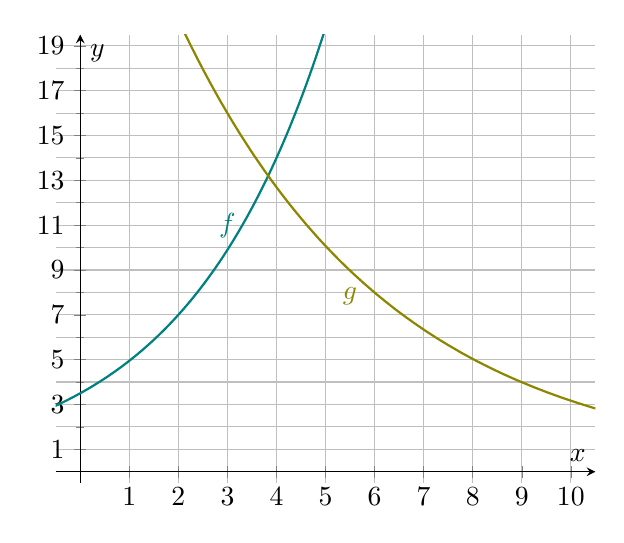
\begin{tikzpicture}
	\begin{axis}[
	axis lines = center, 
	xmin = -0.5, ymin = -0.5,
	xmax = 10.5, ymax = 19.5,
	xtick = {-1,0,1,...,10},
	ytick = {-1,1,...,19},
	grid = both, 
	minor y tick num = 1,
	xlabel = $x$, ylabel = $y$,
	]	
		\addplot[color = teal, thick, domain = -1:11, samples = 200] {3.5*1.4142^x};
		\addplot[color = olive, thick, domain = -1:11, samples = 200] {32*0.79370^x};
		\node[anchor = south, color = teal] at (axis cs: 3,10) {$f$};
		\node[anchor = south, color = olive] at (axis cs: 5.5,7) {$g$};
	\end{axis}
	\end{tikzpicture}
	\caption{Grafer for eksponentialfunktionerne $f$ og $g$.}
	\label{fig:grafer}
\end{figure}
\begin{enumerate}[label=\roman*)]
	\item Aflæs fordoblingskonstanten for $f$ og halveringskonstanten for $g$. 
\end{enumerate}


\subsection*{Opgave 4}
\begin{enumerate}[label=\roman*)]
	\item Bestem $\log_2(256) - \log_3(27).$
	\item Løs ligningen $3^{7x-24} = 81.$
\end{enumerate}

\subsection*{Opgave 5}
To linjer er givet ved
\begin{align*}
	&2x - 4y = 6\\
	&4x + 7y = 3\\
\end{align*}
\begin{enumerate}[label=\roman*)]
	\item Bestem skæringspunktet mellem linjerne. 
\end{enumerate}

\subsection*{Opgave 6}
Parablen for et andengradspolynomium $p$ givet ved
\begin{align*}
	p(x) = ax^2 + bx + c
\end{align*}
kan ses på Figur \ref{fig:parabel}.
\begin{figure}[h]
	\centering
	\begin{tikzpicture}
	\begin{axis}[
		axis lines = center, 
		xmin = -4, xmax = 6, 
		ymin = -12, ymax = 10,
		ticks = none, 
		xlabel = $x$, ylabel = $y$, 
		]
		\addplot[color = teal, thick, samples = 500] {(x+2)*(x-4};
	\end{axis}
	\end{tikzpicture}
	\caption{Parabel for $p$.}
	\label{fig:parabel}
\end{figure}
\begin{enumerate}[label=\roman*)]
	\item Bestem fortegnet på tallene $a$, $b$ og $c$. 
	\item Bestem fortegnet på diskriminanten $d$. 
\end{enumerate}

\subsection*{Opgave 7}
\begin{enumerate}[label=\roman*)]
	\item Løs ligningen $5x^2 + 10x - 15 = 0$. 
	\item Løs ligningen $(x^2-9)(x^2 - 7x -12)$.
\end{enumerate}

\newpage
\subsection*{Opgave 8}
\begin{enumerate}[label=\roman*)]
	\item Aflæs $\cos(134.4)$ ved at bruge følgende enhedscirkel.
\end{enumerate}
\begin{center}
	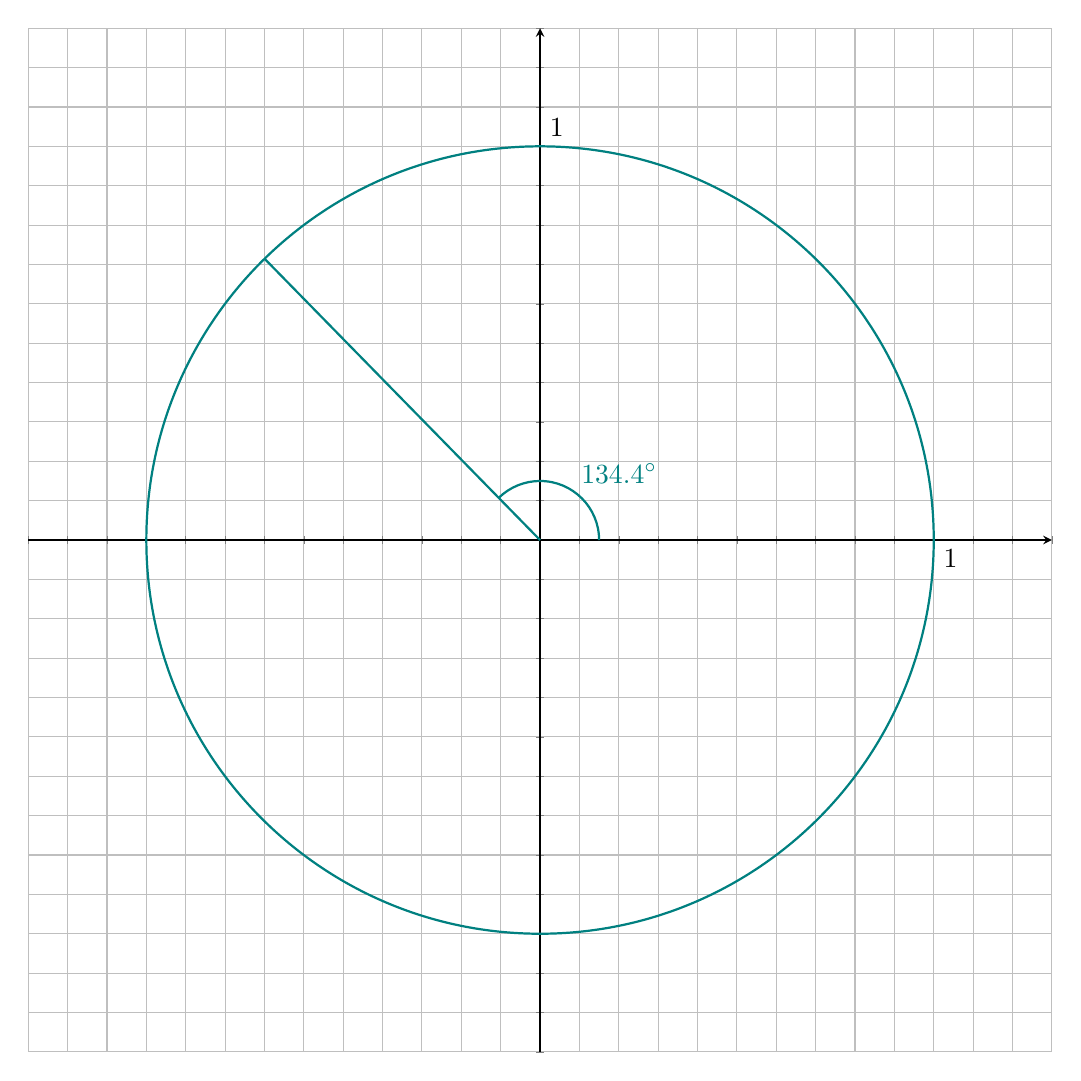
\begin{tikzpicture}
	\begin{axis}
		[
		axis lines = center, 
		xmin = -1.3, xmax = 1.3,
		ymin = -1.3, ymax = 1.3,
		x = 5cm, y = 5cm,
		xtick = {-4,-2,...,2,4},
		ytick = {-4,-2,...,2,4},
		minor tick num = 19,
		grid = both,
		]
		\draw[thick, color = teal] (axis cs: 0,0) circle (5cm);
		\draw[color = teal, thick] (axis cs: 0,0) -- (axis cs: {cos(134.4},{sin(134.4)});
		\draw[color = teal, thick] (axis cs: 0.15,0) arc[start angle = 0, end angle = 134.4, radius = 0.15*5cm];
		\node[color = teal, anchor = south west] at (axis cs: 0.08,0.12) {$134.4^\circ$};
		\node[anchor = north west] at (axis cs: 1,0) {$1$};
		\node[anchor = south west] at (axis cs: 0,1) {$1$};
	\end{axis}
	\end{tikzpicture}
\end{center}

\subsection*{Opgave 9}
Lav trekantsopgaver fra de tidligere moduler - De tager lang tid at lave, så I får pæne tal, så I må lige genbruge fra de tidligere moduler. 

\newpage

\begin{center}
	\Large Med hjælpemidler
\end{center}

\subsection*{Opgave 1}
En potensfunktion $g$ opfylder, at $g(2) = 17$ og $g(5) = 103$
\begin{enumerate}[label=\roman*)]
	\item Bestem en forskrift for $g$. 
	\item Løs ligningen $g(x) = 200$. 
\end{enumerate}

\subsection*{Opgave 2}
\begin{center}
		\includegraphics[width=0.4\textwidth]{Billeder/skolehojde}
	\end{center}
	Højden og vægten er blevet målt for en række elever i skolealderen. Resultatet af målingerne kan findes 
	i \href{https://github.com/ChristianJLex/TeachingNotes/raw/master/2024-2025/Data%20og%20lign/skolevaegt.xlsx}{\color{blue!60}dette datasæt.} 
	Det antages, at sammenhængen mellem elevernes højde og vægt kan beskrives ved en potenssammenhæng. 
\begin{enumerate}[label=\roman*)]
	\item Brug datasættet til at bestemme en forskrift, der beskriver sammenhængen mellem højde og vægt ved regression.
	\item Brug modellen til at bestemme vægten for en elev på 1.10 meter.
\end{enumerate}

\subsection*{Opgave 3}
\begin{center}
		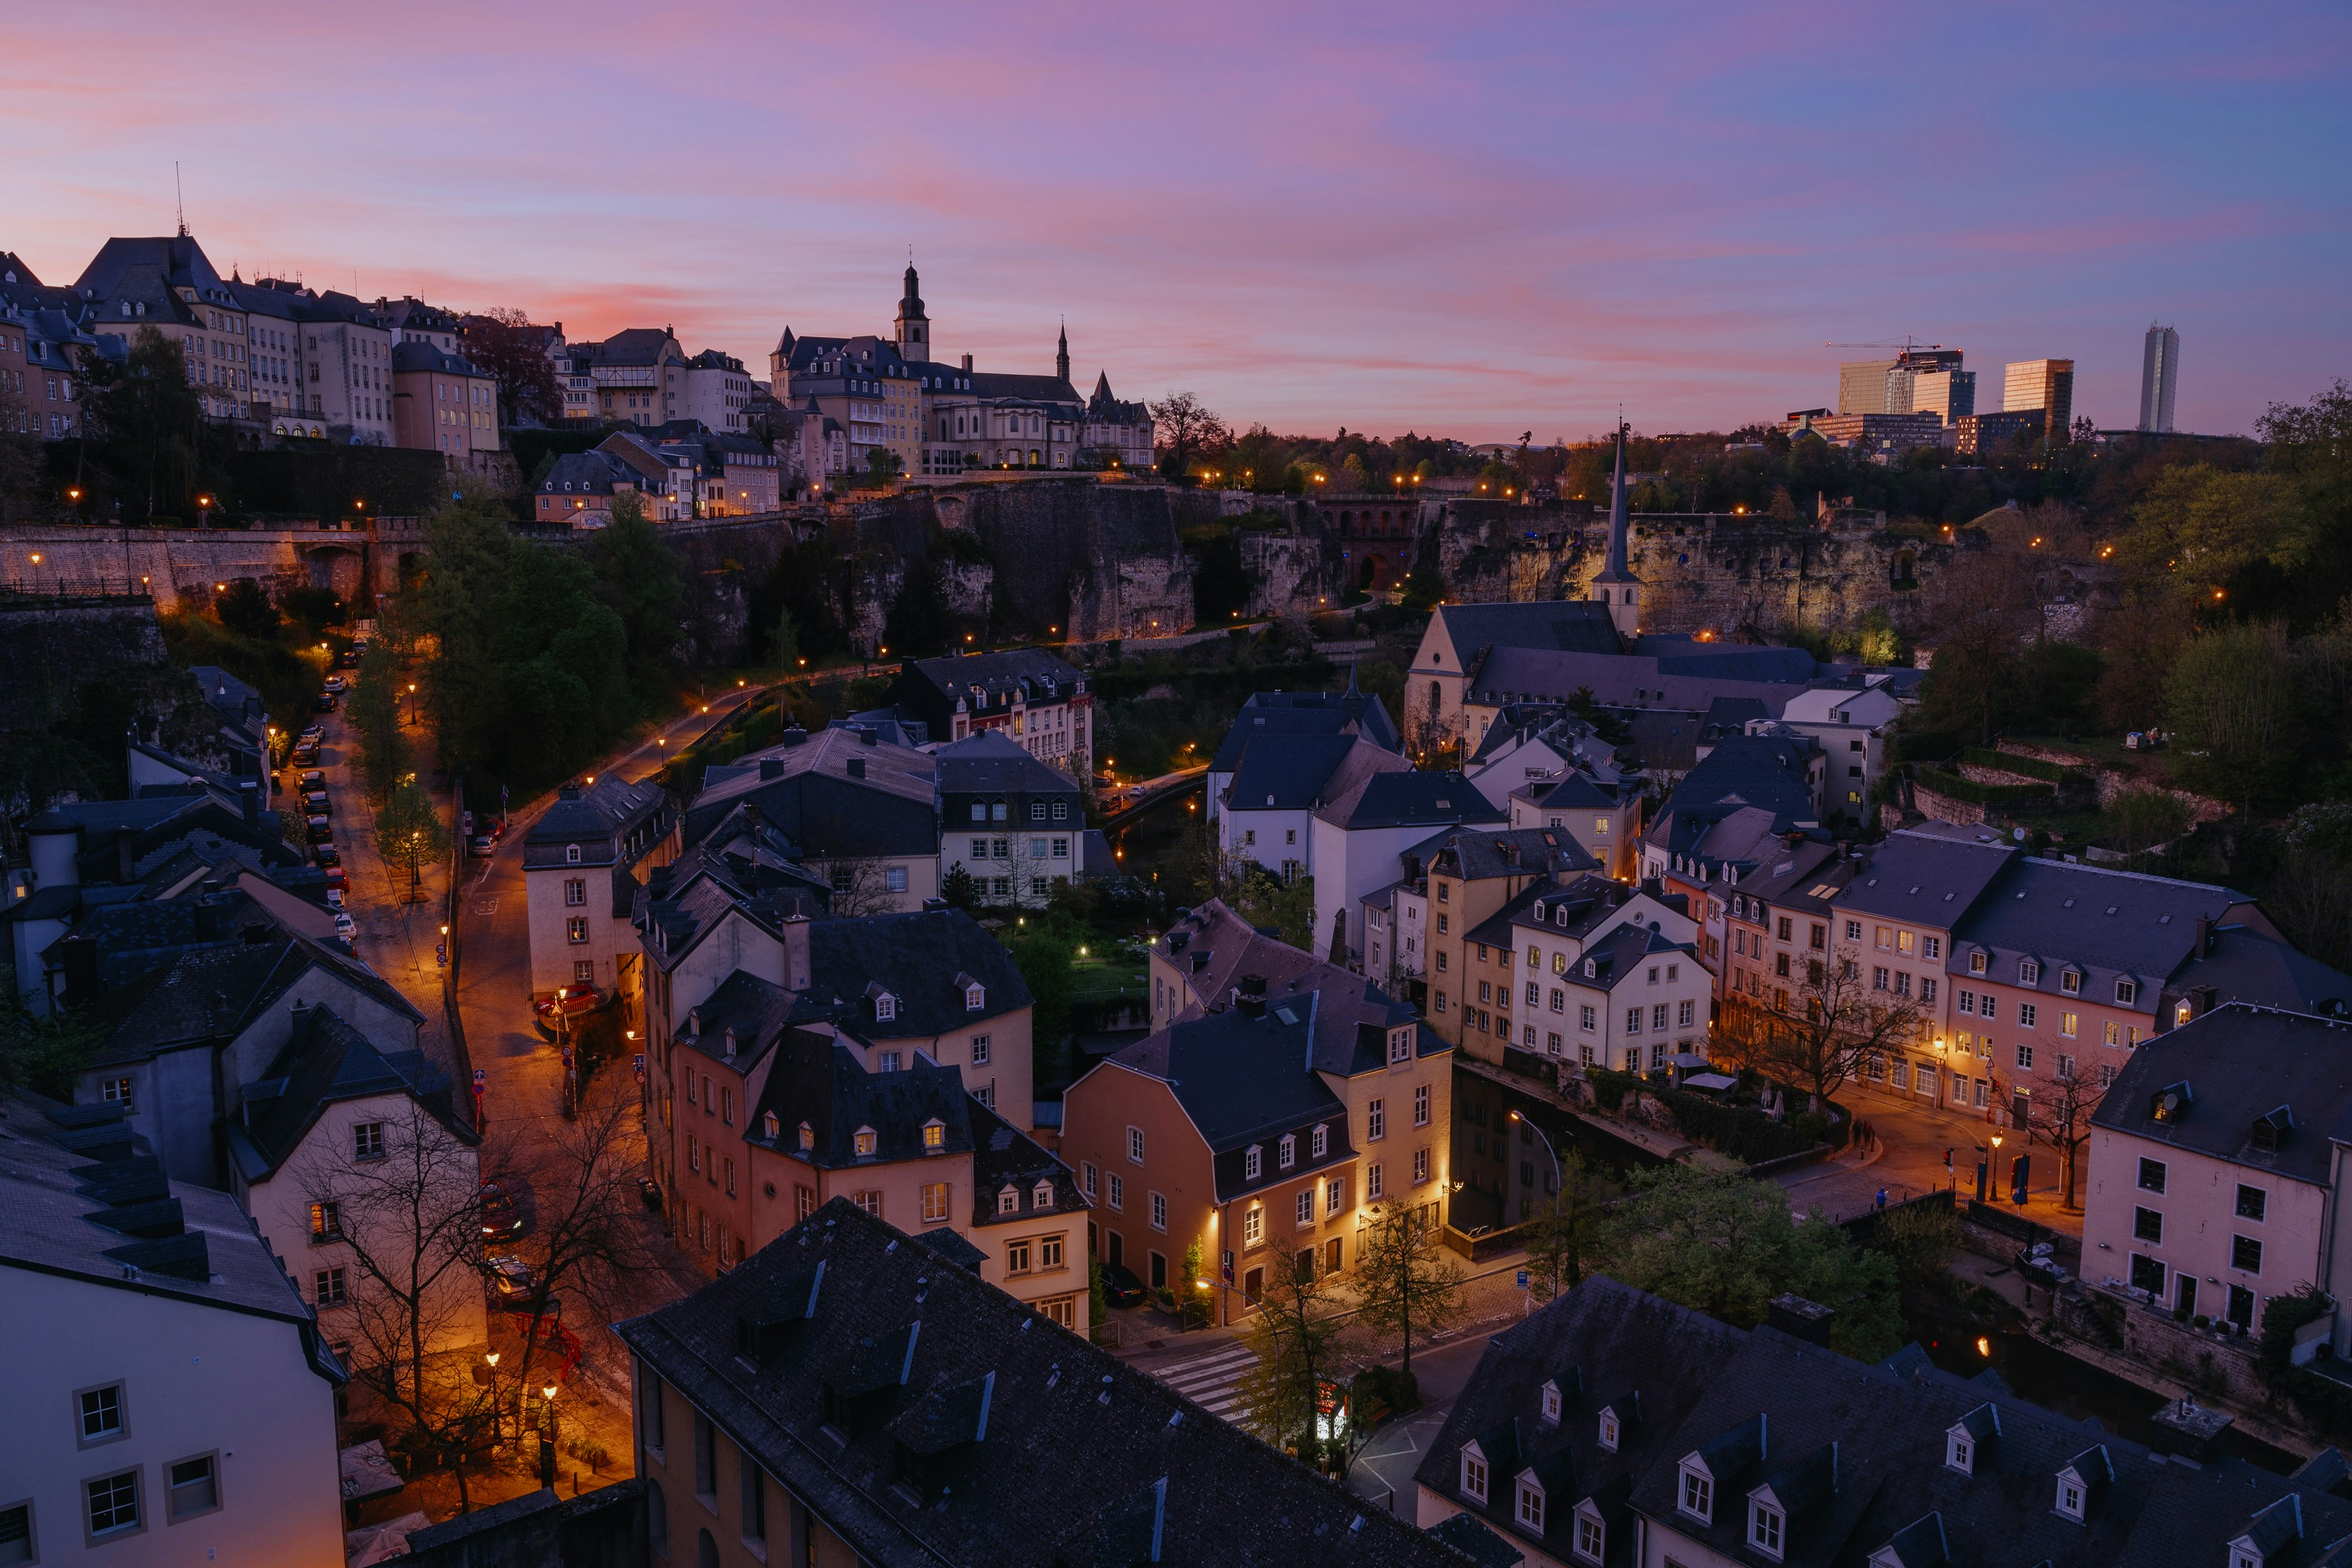
\includegraphics[width=0.5\textwidth]{Billeder/luxembourg}
	\end{center}
	Antallet af beboere i en by kan beskrives ved sammenhængen $f$ givet ved
	\begin{align*}
		f(t) = 2055\cdot 1.03^t,
	\end{align*}
hvor $t$ betegner antal måneder efter år 1996 og $f$ er antal beboere i byen.

\begin{enumerate}[label=\roman*)]
	\item Bestem fordoblingskonstanten for $f$ og forklar, hvad denne betyder for udviklingen af byen.
	\item Bestem det årstal hvor antallet af beboere i byen vil være firedoblet ifølge modellen. 
\end{enumerate}
\newpage

\subsection*{Opgave 4}

En funktion $h$ er givet ved
\begin{align*}
	h(x) = \ln(x) - x^2. 
\end{align*}
\begin{enumerate}[label=\roman*)]
	\item Tegn grafen for $h$ på intervallet $[2,5]$.
\end{enumerate}

\end{document}